\chapter*{Pre-processing}
\stepcounter{chapter}

\section{Combining Attributes and Numerical Data:}
For low instance variables, a manual assignment from numerical values to worded categories was taken. However, in the
cases of large variable assignments it was easier to merge attributes with the appropriate columns in the table and then
prune undesired columns and re-name the new variable columns. For remaining values, Formula widget was used to populate values.
\begin{figure}[H]
    \centering
    \includegraphics[width=0.8\textwidth]{chapters/part 1 - images/Attribute_node_structure.png}
    \caption{Node structure for turning numerical data into attribute values.}
\end{figure}

\section{Outlier and Missing data:}
Using a subset of $5000$ records, the 'Outlier' widget was used to identify and categories outliers. While generally good practice,
there could also exist trends within these extremes themselves; for example, all of these cases could have attended the same level of
education.
\begin{figure}[H]
    \centering
    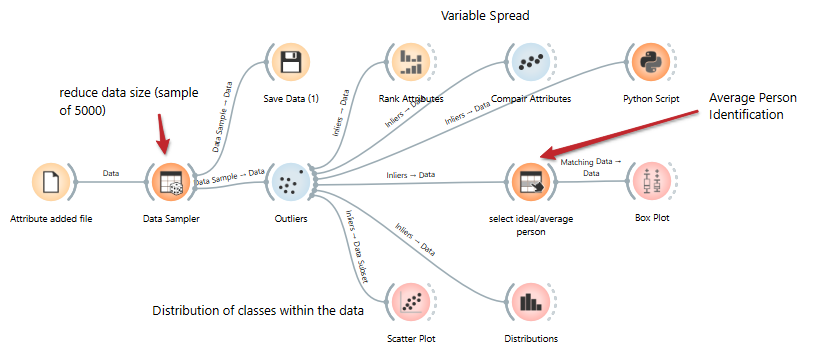
\includegraphics[width=0.8\textwidth]{chapters/part 1 - images/refined_data.png}
    \caption{Identifying and Removing Outliers.}
\end{figure}


\section{Dataset Overview \& Summary Statistics:}
\paragraph{Race} With some minority groups, such as "\texttt{Alaska Native}", with only one representative no general prediction could be made.
As a result, minority groups are combined to form a binary classification of \texttt{White} and \texttt{Not-White}. Similarly,
\textbf{place of birth} was also culminated into \texttt{US} and \texttt{Non-US} to help reduce skewness and maintain data validity.

Frequency distributions necessitated combining groups for statistical robustness. While White participants composed 78\% of the data, the next
largest category was only 9\%. Similarly, all non-US regions combined totaled only ~16\%. Consolidation ensures more reliable comparisons
across categories.

The same is also said for \textbf{education}, with many peoples educational background varying largely based on how long they spent in
school, it is easier to group by their achievements (checkpoints) within this field. Specifically, categories $1 \to 15$ were mapped to
\texttt{no-diploma}, $16 \to 17$ to \texttt{high-school}, and $18 \to 19$ to \texttt{post-high-school}, with subsequent levels representing
higher-tier qualifications.

Finally, the \textbf{Industry} attribute was extracted to identify broader economic trends. Using specific job titles would have
introduced excessive "noise," as identical roles often have varied titles based on company or location. By grouping these into industrial
sectors, the data reveals systemic trends rather than isolated instances.

\subsection{Preliminary Observations}
With the main aim being to predict a persons' \textbf{income}, it is good to establish a baseline to compare to. In this case, it consists
of choosing someone that fits in to the most common category. Following from the data refinement, the most common person consists of
someone:
\begin{itemize}
    \item \textbf{White}
    \item \textbf{Married}
    \item Works in an \textbf{Office}
    \item Achieved qualifications \textbf{Post High-school}
\end{itemize}
, this person earns anywhere from $\$21,000\to\$70,000$. However, the mean income for someone with all of these attributes is
$\$62,881.25$; way above the expected $\$39,000$. This large deviation is a result of positive skewness within the demographic,
where a minority of high-earners pulls the average upward, misrepresenting the typical individual. To
mitigate this, the following analysis linearises the relationship between attributes and earning, allowing for a more accurate
comparison.